\chapter{A Domain Specific Language for Legal Agreements}\label{ch:lang}

One of the key focuses of this project is not just to be able to represent legal contracts with specific properties and capabilities as described in~\autoref{ch:queries};
but also to make it as easy as possible for people with non-technical backgrounds to use such representations.
Simply put, a lawyer should not need to learn JSON.

This is the main motivation for developing tooling which aims to make it easier for people of non-technical backgrounds to produce, modify, and understand Confis legal agreement representations.
The core of this tooling is the Confis language~(\autoref{sec:developing-a-dsl}) and an IDE-assisted editor~(\autoref{sec:confis-editor}).


\section{Motivations For a DSL}\label{sec:developing-a-dsl}

\subsection{Implementation Requirements}\label{subsec:dsl:requirements}

The language should fulfil the core requirements set out in~\autoref{ch:evaluation}.
This involves prioritising~\nameref{def:accessibility} while making sure~\nameref{def:completeness} and~\nameref{def:soundness} are possible.

\subsubsection{Easy to write while still machine-readable}

Writing a Confis agreement should be close to writing plain English, while still being machine-readable.
For more details on the meaning of \emph{machine-readable} in the context of this project, see~\autoref{sec:machine-readable-contracts}.


A compromise must be struck between ease of writing and machine-readability.

\paragraph{Data Serialization Language}

On one extreme, a data serialization text file (like JSON, YAML, or XML) would allow writing text that can be easily parsed by a program.
But writing such files requires some data structures knowledge;
and because of their key-value nature they do not allow writing sentences, leaving them too far from the readability of human-written legal prose -- thus they lack the~\nameref{def:accessibility} property.

\paragraph{Natural Language Processing}

On the other extreme, legal prose processed through a language processing program allows the drafter to completely ignore the machine-readable aspect of the document.
Readers would be able to integrate such documents in their existing workflows -- as they would need to make no transition from their existing, non-machine-readable documents.
This is approach is discussed in~\autoref{sec:nlp} -- we conclude it does not meet the~\nameref{def:completeness} property.  \\

A compromise between these two solutions would be a language formal enough that it can be parsed by a program, but natural enough that natural language sentences can be recognised in it.
Python or AppleScript~\cite{Sanderson2010appleScript}~(see~\autoref{fig:appleScript}) are good examples of programming languages (and therefore parseable) that are engineered with the goal of resembling English as much as possible.

\begin{listing}[h]
    \centering
    \begin{minipage}{0.8\textwidth}
        \begin{minted}[
            autogobble,
            frame=lines,
            framesep=2mm
        ]{applescript}
                set the firstnumber to 1
                set the secondnumber to 2
                if the firstnumber is equal to the secondnumber then
                    set the sum to 5
                end if
        \end{minted}
    \end{minipage}
    \caption{Sample code snippet of the AppleScript Language~\cite{Sanderson2010appleScript}}
    \label{fig:appleScript}
\end{listing}

\subsubsection{Easy to develop and extend}

With pragmatic implementation efforts in mind, this project should not aim to develop its own parser and interpreter or compiler: the project hopes to be more concerned with introducing a suitable abstraction that allows both drafting and processing legal documents.

\subsubsection{Additional tooling for ease of use and correctness}

A key aspect of development for a new user of a language is to understand the concepts of syntax, compile errors, and invalid programs.
A great aid to developing this understanding are visual cues in editors in integrated development environments (or IDEs).

For the Confis DSL to be successful, it must be easy for the drafter of legal agreements to reason about the correctness of the document within the formalisms set out by this project.
Good tooling is therefore a key requirement in order to achieve~\nameref{def:accessibility}.

\subsection{Implementation Requirements Conclusion}\label{subsec:dsl-design-conclusion}

The requirements of~\autoref{subsec:dsl:requirements} lead to the following design choices:

\paragraph{A Textual Domain-Specific Language} For a good compromise between readability, flexibility and rigidity of the agreements that can be written, this project therefore proposes developing a DSL~(see~\nameref{sec:dsls}) as a suitable compromise that allows working with a human-readable encoding which can then be compiled to a suitable machine-readable representation.

We will call this language \textbf{\emph{Confis DSL}} (or \emph{Confis language}) and the machine-readable representation it compiles to \textbf{\emph{Confis Internal Representation}} (or \emph{Confis IR}).
The Confis IR will be used for processing as discussed in~\autoref{ch:queries}.

\paragraph{An Internal DSL}
For the sake of development costs, we use a suitable host language to implement the Confis DSL (as opposed to developing an external DSL).

\paragraph{A separate Internal Representation}
Another key design decision is to develop the internal representation (the Confis IR) separately from the DSL\@.
By `develop separately' we mean that the internal representation should be enough to represent an agreement, and it should be possible to construct it independently of the Confis DSL\@.
% TODO discuss in future work
This should allow developing a stand-alone language as an external DSL (or alternatively, a graphical DSL or a new internal DSL in some other host language) in the future that utilises the same Confis IR -- thus preserving the formalisms this project contributes in this new language.

\paragraph{Kotlin as a host language} Several host languages can serve to build a DSL.
A few options are discussed in~\autoref{subsec:dsl-host-candidates}, like Groovy and Haskell.
The choice to use Kotlin stems from how feature-rich the surrounding tooling is -- such as its stand-alone custom scripting~\cite{kotlinScriptKeep} and IDE support~\cite{intelliJRepo}.


\section{Language Semantics and Design}\label{sec:language-semantics}

This section is concerned with the structure, semantics, and design decisions regarding the Confis DSL.
For the implementations details of the DSL, see~\nameref{subsec:dsl-implementation}.
For motivations and priorities of the project, see~\nameref{sec:eval:goals}.

%Given decoupling the Confis language and the Confis IR is a requirement as discussed in~\autoref{subsec:dsl:requirements}, the language

% TODO come back after doing reasoning background
Confis introduces the following formalisms in order to limit the complexity of the language.

\begin{definition}[Party]
    \label{def:party}

    A \emph{Party} to the agreement is a legal person (a real person, an institution, a company, or even a group of people).
    Parties are unique in an agreement and are identifiable by a name (encoded as a UTF-8 string).
\end{definition}

\begin{definition}[Action]
    \label{def:action}
    An \emph{Action} represents something that can be initiated by a Party.
    It is unique in an agreement and is identifiable by a name (encoded as a UTF-8 string).
\end{definition}

\begin{definition}[Thing]
    \label{def:thing}
    A \emph{Thing} is unique in an agreement and is identifiable by a name (encoded as a UTF-8 string).
    An Thing resembles a~\nameref{def:party} but it does not aim to represent a legal person and it cannot be a subject on a~\nameref{def:sentence}.
\end{definition}

A Sentence is the building block of a Confis agreement.
It is combined with other elements in order to form clauses and, combined with a Circumstance Set, it forms an event that includes a context.

\begin{definition}[Sentence]
    \label{def:sentence}
    A \emph{Sentence} is a tuple like~\texttt{Sentence = (Subject, Action, Object)}, where a \texttt{Subject} is a~\nameref{def:party} and \texttt{Object = Party | Thing}.
\end{definition}

Allowance is used to answer questions of the type \emph{`May A do X?'} -- where \emph{yes} or \emph{no} are not enough to model all the possibilities given in the legal domain.


\begin{definition}[Allowance]
    \label{def:allowance}
    \emph{Allowance} is a value like \texttt{Allowance = Allow | Forbid | Unspecified | Depends}.
\end{definition}

Users are allowed to use Allowance in order to define a~\nameref{def:permission}, but only the values \texttt{Allow} and \texttt{Forbid}.
The other values are reserved for answering queries and while they cannot be used, responses that return \texttt{Depends} and \texttt{Unspecified} can be crafted by defining the answer space accordingly.
This is shown in~\autoref{fig:allowance-venn} and~\autoref{eq:allowance-cake-example}, where only \texttt{may} and \texttt{mayNot} keywords are used (corresponding to \texttt{Allow} and \texttt{Forbid} respectively) but all possible values of Allowance are present in the agreement.

\begin{figure}[h]
    \centering
    \begin{minipage}{0.5\textwidth}
        \begin{minted}[
            autogobble
%            frame=lines,
%            framesep=2mm
        ]{kotlin}
            val alice by party
            val eat by action
            val cake by thing

            alice may eat(cake) asLongAs {
                with purpose Research
            }
            alice mayNot eat(cake) asLongAs {
                with purpose Commercial
            }
        \end{minted}
    \end{minipage}

    \vspace{0.2cm}

    \begin{tikzpicture}
        \node [
%        draw,
        circle,
        fill=gray,
        minimum size =5cm,
        label={135:$\text{alice eat cake}$}] (Eat) at (1.25,0){};

        \node [
%        draw,
        circle,
        fill=mdtGreen,
        minimum size =2.5cm,
        label={180:$\text{\small with purpose Research}$}] (A) at (0,0){};

        \node [
%        draw,
        circle,
        fill=mdtRed,
        minimum size =2.5cm,
        label={0:$\text{\small with purpose Commercial}$}] (B) at (2.5,0){};

        \node[white] at (0, 0) {\texttt{Allow}};
        \node[white] at (2.5, 0) {\texttt{Forbid}};
        \node[white] at (1.25, 1.5) {\texttt{Depends}};
        \node at (5, 1.5) {\texttt{Unspecified}};

    \end{tikzpicture}

    \caption{Agreement and Venn Diagram of a `\texttt{alice eat cake}?' query}
    \label{fig:allowance-venn}
\end{figure}

\begin{align}
    \label{eq:allowance-cake-example}
    \text{alice eat cake?} &\to \texttt{Depends}\\
    \text{alice eat cake with purpose Research?} &\to \texttt{Allow}\\
    \text{alice eat cake with purpose Commercial?} &\to \texttt{Forbid}\\
    \text{alice eat cake with purpose Internal?} &\to \texttt{Unspecified}
\end{align}


\begin{definition}[Permission]
    \label{def:permission} A \emph{Permission} represents a legal capability (or lack thereof) in the language.
    It is a tuple of a~\nameref{def:sentence}, an~\nameref{def:allowance}, and a~\nameref{def:circumstanceSet} (which may be empty).
    \begin{verbatim}
        Permission = (Sentence, Allowance, CircumstanceSet)
    \end{verbatim}
\end{definition}

A requirement is an important abstraction necessary in order to define~\nameref{def:confis-compliance}.
Confis also assumes a that providing a legal obligation entails providing the legal capability to fulfill that obligation, which means that when we have a Requirement we have an \texttt{Allow} Permission too.

\begin{definition}[Requirement]
    \label{def:requirement} A \emph{Requirement} represents a legal obligation and is a tuple of a~\nameref{def:sentence} and a~\nameref{def:circumstanceSet} (which may be empty).
    \begin{verbatim}
        Requirement = (Sentence, CircumstanceSet)
    \end{verbatim}

    A requirement $r$ entails a permission $p$ where if $r = (s, C)$ then $p = (\texttt{Allow}, s, C)$
\end{definition}

\begin{definition}[Event]
    \label{def:event}
    An \emph{Event} is a tuple of a Sentence and a Circumstance set, describing the context the Sentence happens in, like \texttt{Event = (Sentence, CircumstanceSet)}
\end{definition}

We use a set of Events to represent a `state-of-the-world'.
Note how we have no concept of precedence or ordering between events.
The only way to order chronologically them would be with respect to a time-based Circumstance present in each event's Circumstance Set.

\begin{definition}[Compliance]
    \label{def:confis-compliance}
    We say that a Requirement $r$ \emph{has been met by} a set of Events $W$ if and only if there is an event $e \in W$ such that they have the same Sentence and the Circumstance Set of $e$ is generalised by the Circumstance Set of $r$.

    We say that a \texttt{Forbid} Permission $p$ \emph{is respected by} a set of Events $W$ if and only if there does not exist $e \in W$ such that $e$ has the same Sentence as $p$ and the Circumstance Set of $e$ overlaps with the Circumstance Set of $p$.

    A set of Events $W$ \emph{is compliant with} an agreement if and only if, for every Requirement $r$ and every \texttt{Forbid} Permission $p$ that are part of the agreement, $r$ has been met by $W$ and $p$ is respected by $W$.
\end{definition}

For the meanings of `generalises' and `overlaps with', see~\autoref{def:circumstanceSet:generalise}, and~\autoref{def:circumstanceSet:overlap}.

\subsection{Circumstance and Circumstance Set}\label{subsec:circumstance}

Circumstances are a core abstraction in Confis, both in the language and in~\nameref{sec:rule-generation} (hence why they deserve their own section).

A Circumstance Set represents the context in which a~\nameref{def:sentence} may occur.
In the context of a legal agreement, it would contain everything in a clause that is not the core sentence, including the parent clause, conditions, etc.

A Circumstance Set is made up of Circumstances.


\begin{definition}[Circumstance]
    \label{def:circumstance}
    $c$ is a \emph{Circumstance} if and only if it is equipped with the following operations for any other circumstance $c'$:
    \begin{align}
        \label{def:c:generalise}
        \texttt{generalise}&: \ c \to\ c' \to\ \texttt{Boolean}\\
        \label{def:c:provideKey}
        \texttt{provideKey}&: \ c \to\ k\\
        \label{def:c:overlap}
        \texttt{overlapsWith}&:\ c \to\ c' \to\ \texttt{Boolean}\\
        \label{def:c:render}
        \texttt{render}&: \ c \to\ \texttt{String}
    \end{align}
\end{definition}

A circumstance key $k$ is simply an element with a notion of equality.
When two circumstances $c_1$ and $c_2$ produce they same key $k$, they are said to be~\emph{of the same type}.
\texttt{render} is a function made to satisfy the requirement of being able to convert a Confis agreement into readable English for the sake of~\nameref{def:accessibility}.

A Circumstance Set is an indexed set of~\nameref{def:circumstance}s, unique in that only one circumstance of each type can be stored.
For example, we can only store a single circumstance representing time and a single circumstance representing purpose, because these are implemented to produce the same key $k$ each.

\begin{definition}[Circumstance Set]
    \label{def:circumstanceSet}
    A \emph{Circumstance Set} is a key-value mapping of Circumstance Keys to \nameref{def:circumstance}, like $\texttt{CircumstanceSet} = \{ k \to \texttt{Circumstance} \}$.
\end{definition}

Defining \texttt{generalise} for circumstances will be of use when trying to define rules (see~\autoref{sec:rule-generation}) because it will allow checking whether a circumstance from a clause `matches' that of a question~(see~\nameref{subsubsec:circumstances-intuition} for an explanation).

\begin{definition}[Circumstance Set Generalisation]
    \label{def:circumstanceSet:generalise}
    Fot two Circumstance Sets $C_1$ and $C_2$ we say $C_1$ \emph{generalises} $C_2$ if and only if:
    \begin{equation}
        \label{eq:circumstanceSet:generalisation}
        \forall k \, \forall c_1.[ \, (k, c_1) \in C_1 \to
        \exists c_2.((k, c_2) \in C_2  \land\ c_1\ \texttt{generalises}\ c_2)\,]
    \end{equation}

    That is, if for all circumstances in $C_1$, there is a circumstance of the same type in $C_2$ and each circumstance in $C_1$ generalises the circumstance of the same type in $C_2$.
\end{definition}

\begin{definition}[Circumstance Set Overlap]
    \label{def:circumstanceSet:overlap}
    For any two Circumstance Sets $C_1$ and $C_2$, we say $C_1$ \emph{overlaps with} $C_1$ if and only if
    \begin{equation}
        \label{eq:circumstanceSet:overlap}
        \forall k \, \forall c_1.[ \, (k, c_1) \in C_1 \to
        \exists c_2.((k, c_2) \in C_2  \land\ c_1\ \texttt{overlapsWith}\ c_2)\,]
    \end{equation}
    That is, if for all circumstances in $C_1$, there is a circumstance of the same type in $C_2$ and each circumstance in $C_1$ overlaps with the circumstance of the same type in $C_2$.
\end{definition}

This definitions of Circumstance Set Generalisation and Overlap have the following consequences:
\begin{itemize}
    \item The empty circumstance set generalises all circumstance sets
    \item The empty circumstance set overlaps with all circumstance sets
\end{itemize}


Although nothing requires Circumstance Set overlap to be commutative, it will be commutative if the Circumstances it contains have a commutative implementation of \texttt{overlapsWith}.
This is the case for every Circumstance built into Confis so far.

\subsubsection{Intuition Behind Circumstances}\label{subsubsec:circumstances-intuition}

Circumstance Sets can be thought of as contexts for a sentence, which together constitute an event.
Defining overlaps and generalisations between these contexts allows us to reason about the same concepts for events: is \emph{`Pay Bob during the month of June'} more general than \emph{`Pay Bob the 10th of June'}? Defining a time range (a day in June, a month within a year) as a Circumstance allows us to answer those questions programmatically.

The empty circumstance set can be thought of as the least specific context for an event (think of it as \emph{anywhere} when thinking about a place).
Indeed, the event \emph{`Alice pays Bob'} generalises the event \emph{`Alice pays Bob during June'}.
If a contract has a requirement for the former, and we supply it with a state of the world containing the latter, we can say that Alice is compliant with the contract!

Likewise, the converse is true for \emph{disjoint} (not overlapping) events.

For two events $e_1 = \textit{`Alice pays Bob during June'}$,  $e_2 = \textit{`Alice pays Bob during September'}$, we can say the Circumstance Sets of $e_1$ and $e_2$ are disjoint, therefore if a contract requires $e_1$ but we have a state of the world with $e_2$, we can say Alice still has some legal obligation she has not fulfilled.

Generally, Circumstance Sets describe more specific situations the more elements they have.
How different Circumstance Sets can overlap and generalise each other is shown by example through the definitions of the sets $A$, $B$, $C$, $D$ and $E$ below.

\begin{align}
    A &= \{ \texttt{time} \to \text{`10th of June 2022 - 12th of June 2022'} \}\\
    B &= \{ \texttt{time} \to \text{`1st of June 2022 - 31st of June 2022'} \}\\
    C &= \{ \texttt{purpose} \to \text{`Commercial'} \}\\
    D &= A \cup C\\
    E &= \{ \texttt{time} \to \text{`1st of June 2022 - 11th of June 2022'} \}
\end{align}

% TODO this is wrong fix it
We have:
\begin{itemize}
    \item The empty Circumstance Set $\emptyset$ generalises and overlaps with $A$, $B$, $C$, $D$ and $E$
    \item $B$ generalises $A$ and $E$
    \item $A$ overlaps with $B$, $D$ and $E$
    \item $B$ overlaps with $A$, $D$ and $E$.
    \item $D$ overlaps with $A$, $B$, $C$, and $E$.
    \item $E$ overlaps with $B$, $D$ and $A$
    \item $C$ overlaps with $D$
\end{itemize}

\subsection{DSL Implementation}\label{subsec:dsl-implementation}

This subsection is concerned with the implementation details of the Confis DSL.
For design decisions regarding the language (like what is a Sentence or the difference between a Requirement and a Capability) please see~\nameref{sec:language-semantics}.

Because of the nature of internal DSLs~(see~\autoref{sec:dsls}), the syntax of the Confis DSL must be a subset of the Kotlin language's.
% TODO add future work link for own lang
Given the Confis DSL and the Confis IR are decoupled this section will not go into too much detail on how the DSL is implemented as most of that is specific to the Kotlin language, and the DSL could have been implemented as an internal DSL with a different host language anyway (like Haskell or Groovy).
Instead, it will show a couple examples of how language constructs are implemented (like a Permission) which will be useful to understand~\autoref{subsec:editor-implementation}.

For more information on how DSLs can be built in Kotlin in general, see~\autoref{subsubsec:kotlinLang}, and in particular refer to~\cite{kotlinTypeSafeBuilders}.

\subsubsection{Permission Builder Implementation}

Recall a~\nameref{def:permission} is a tuple of~\texttt{(Allowance, Sentence, CircumstanceSet)}, where the \texttt{CircumstanceSet} may be empty.
For the sake of brevity, we will leave the construction of the Circumstance Set out and discuss how we can construct a tuple of \texttt{(Allowance, Sentence)} in the DSL.
% TODO CircumstanceMap
First, we must define the tuple for~\nameref{def:sentence} in Kotlin as in~\autoref{fig:kotlinSentence}.
Recall a \texttt{Sentence} is simply a tuple of \texttt{(Subject, Action, Object)}.

\begin{listing}[h]
    \centering
    \begin{minipage}{0.4\textwidth}
        \begin{minted}[
            autogobble,
            frame=lines,
            framesep=2mm]{kotlin}
        data class Sentence(
            val subject: Subject,
            val action: Action,
            val obj: Object,
        )
        \end{minted}
    \end{minipage}
    \caption{\texttt{Sentence} tuple declaration}\label{fig:kotlinSentence}
\end{listing}

We now need a DSL to construct this \texttt{Sentence}.
We use an infix extension function in order to add the \texttt{`may'} adverb (which corresponds to \texttt{Allowance = Allow}) between the subject and the action of the sentence (\autoref{fig:permissionKotlin}).

\begin{listing}[h]
    \centering
    \begin{minipage}{\textwidth}
        \begin{minted}[
            autogobble,
            frame=lines,
            framesep=2mm]{kotlin}
        // <Action, Object> tuple declaration
        data class ActionObject(val action: Action, val obj: Object)

        infix fun Subject.may(s: ActionObject) {
            val permission = Permission(Allow, Sentence(this, s.action, s.obj))
            clauses += permission
        }
        \end{minted}
    \end{minipage}
    \caption{Extension function to build a Permission}\label{fig:permissionKotlin}
\end{listing}



\begin{listing}[h]
    \centering
    \begin{minipage}{0.5\textwidth}
        \begin{minted}[
            autogobble,
            frame=lines,
            framesep=2mm]{kotlin}
            val alice: Subject
            val eat: Action
            val cake: Object

            alice may ActionObj(eat, cake)
        \end{minted}
    \end{minipage}
    \caption{Invocation of Permission builder from~\autoref{fig:permissionKotlin}}
    \label{fig:permissionUse}
\end{listing}

Now~\autoref{fig:permissionUse} almost reads like English, except the constructor of the tuple class \texttt{ActionObj}.
We can use a Kotlin operator function in order to overload the \texttt{Action}, so the user is able to write \texttt{action(object)} as opposed to \texttt{ActionObj(action, obj)}.
The full example is demonstrated in~\autoref{fig:permissionKotlinFull}, and a usage example is given in~\autoref{fig:finalPermissionInvocationDSL} -- which now reads much more like an English sentence!


\begin{listing}[h]
    \centering
    \begin{minipage}{\textwidth}
        \begin{minted}[
            autogobble,
            frame=lines,
            mathescape,
            framesep=2mm]{kotlin}
            // <Action, Object> tuple declaration
            data class ActionObject(val action: Action, val obj: Object)

            // this easily builds an ActionObject
            // action.invoke(obj) == action(obj)
            operator fun Action.invoke(obj: Object) = ActionObj(this, obj)

            infix fun Subject.may(s: ActionObject) {
                val permission = Permission(Allow, Sentence(this, s.action, s.obj))
                clauses += permission
            }
        \end{minted}
    \end{minipage}
    \caption[Finished Permission builder]{Finished Permission builder with operator overloading (see~\cite{kotlinInvokeOperator})}
    \label{fig:permissionKotlinFull}
\end{listing}



\begin{listing}[h]
    \centering
    \begin{minipage}{0.5\textwidth}
        \begin{minted}[
            autogobble,
            frame=lines,
            framesep=2mm]{kotlin}
            val alice: Subject
            val eat: Action
            val cake: Object

            alice may eat(cake)
        \end{minted}
    \end{minipage}
    \caption{Example of the DSL invocation of the final Permission builder of~\autoref{fig:permissionKotlinFull}}
    \label{fig:finalPermissionInvocationDSL}
\end{listing}

We now can call the function \texttt{may()} in order to create a \texttt{Permission} and add it to \texttt{clauses}.
Most of the Confis DSL is implemented similarly.
An advantage of using a statically typed language for a DSL with well-defined types like in the examples given above means that only semantically correct sentences can be written.
For example, \texttt{`cake may eat(alice)'} produces a compilation error, because \texttt{`cake'} is not a \texttt{Subject}.


% TODO is this worth writing about at all


\section{Additional Tooling: Legal Prose Rendering}\label{sec:additional-tooling:doc-rendering}

In order to comply with the~\nameref{def:accessibility} requirement, it should be possible to generate a traditional document (perhaps in plaintext or PDF format) written in legal prose.
This generated document should then be usable in place of traditional agreement documents -- for example, a reviewer of an agreement will not need Confis software or to know about the Confis DSL in order to read a copy of the contract.

We will call this feature \textbf{\emph{legal prose rendering}}.

If NLP~(see~\autoref{sec:nlp}) aims to translate traditional human-written legal-prose into a machine-readable format, you can think of legal prose rendering as the inverse process: we go from a machine-readable representation to a more human-readable one.

% TODO

\section[The Confis Editor]{Additional Editing Tooling: the Confis Editor}\label{sec:confis-editor}

One of the key requirements for Confis is~\nameref{def:accessibility}.
In order to achieve this the Confis framework includes an extension to the IntelliJ Development Environment~\cite{intelliJRepo} - the \textbf{\emph{Confis Plugin}}.
Bundled with this plugin is the \textbf{\emph{Confis Editor}}.

The Confis Editor has two main goals:

\paragraph{Providing context-aware aid for authoring agreements} Much like an IDE provides relevant aid to a software engineer (such as reporting compile errors before attempting to compile the program) the Confis Editor should allow an agreement drafter to write in the Confis DSL without needing to deal with command-line utilities or knowing the tooling around Kotlin language.

\paragraph{Providing a human-readable preview of the Confis Agreement}

The Confis Editor should display a document in legal prose, made up from text generated from the Confis agreement (thanks to legal prose rendering~\ref{sec:additional-tooling:doc-rendering}).
This preview should resemble a traditional legal document, and appear side-to-side the code the agreement drafter is writing in order to provide a useful live preview of the contract being authored (much like it is handy to have a PDF preview when drafting TeX documents).

\subsection{Editor Implementation}\label{subsec:editor-implementation}

Two things are required in order to be able to draft single Confis code files inside an IDE:
\begin{enumerate}
    \item It must be possible to write a self-contained, boilerplate-free contract in a single file.
    \item The IDE must perform reporting specific to the Confis DSL when editing this file (as opposed to reporting on the host language, Kotlin).
\end{enumerate}

(1.) is where Kotlin's custom scripting support~\cite{kotlinScriptKeep} is crucial.
See~\nameref{subsec:scripting-support} for a discussion on what is meant by scripting and how it is required for making a stand-alone DSL.

In order to implement writing Confis agreements as stand-alone files, we create a \emph{Kotlin Custom Script definition}~\cite{kotlinScriptKeep}, which essentially contains information that assigns an instance of a class to a script.
By placing DSL builder functions like those introduced in~\autoref{fig:permissionKotlinFull} inside a class (called \texttt{AgreementBuilder}, for example) and assigning an instance of this class to a script, we can let the script author (ie, the Confis agreement author) \textbf{mutate} our class when we evaluate their script.

See~\autoref{fig:agreementBuilderSmall} for an example of such a class, and~\autoref{fig:confis:minimal} for an example of a single script bound to that class.

We can then pass the script definition mentioned above to an extension point present in the IntelliJ API engineered specifically for this purpose~\cite{ideaExtensionPoints, intelliJRepo}.
If we include some additional information (such as a file extension for Confis agreements) IntelliJ will now provide visual hints for Confis Scripts.

\begin{figure}[h]
    \centering
    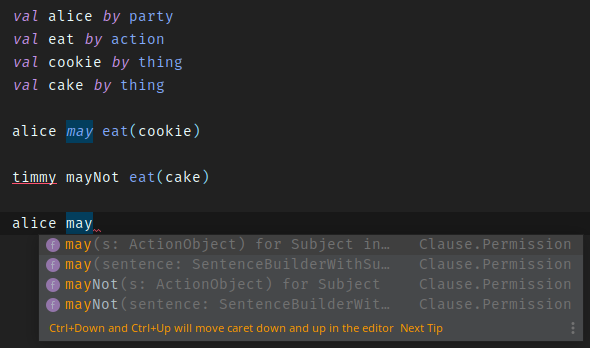
\includegraphics[width=0.75\textwidth]{figures/minimal.editor.highlighting.confis}
    \caption{Syntax highlighting in a small Confis agreement}
    \label{fig:intelliScriptAid}
\end{figure}

See~\autoref{fig:intelliScriptAid} for an example where the Confis editor reports a compile error (where the user attempted to form a Sentence with a Party that does not exist) as well as autocompletion for building a Permission clause.
% TODO actually do this on the website
A live video example can be found in the~\href{https://confis.dcotta.eu/0.1.1/IDE%20Support/IDEAPlugin/}{Confis Documentation Page}.

In order to achieve (2.), we can implement a new editor in IntelliJ based on its existing markdown editor~\cite{ideaMarkdownPreview} which achieves a very similar purpose: providing a live preview of machine-readable code.

The live preview is implemented as a preview of an in-memory Markdown document which is in turn generated upon code changes in the editor:
\begin{equation*}
    \text{Confis Code}\; \to\; \text{Confis IR}\; \to\; \text{Markdown document}\; \to \text{HTML page}\; \to\; \text{Live preview}
\end{equation*}

A screenshot of the Confis Editor, including syntax highlighting and the live preview, can be found in~\autoref{fig:confis.minimal.editor}.

\begin{figure}[h]
    \centering
    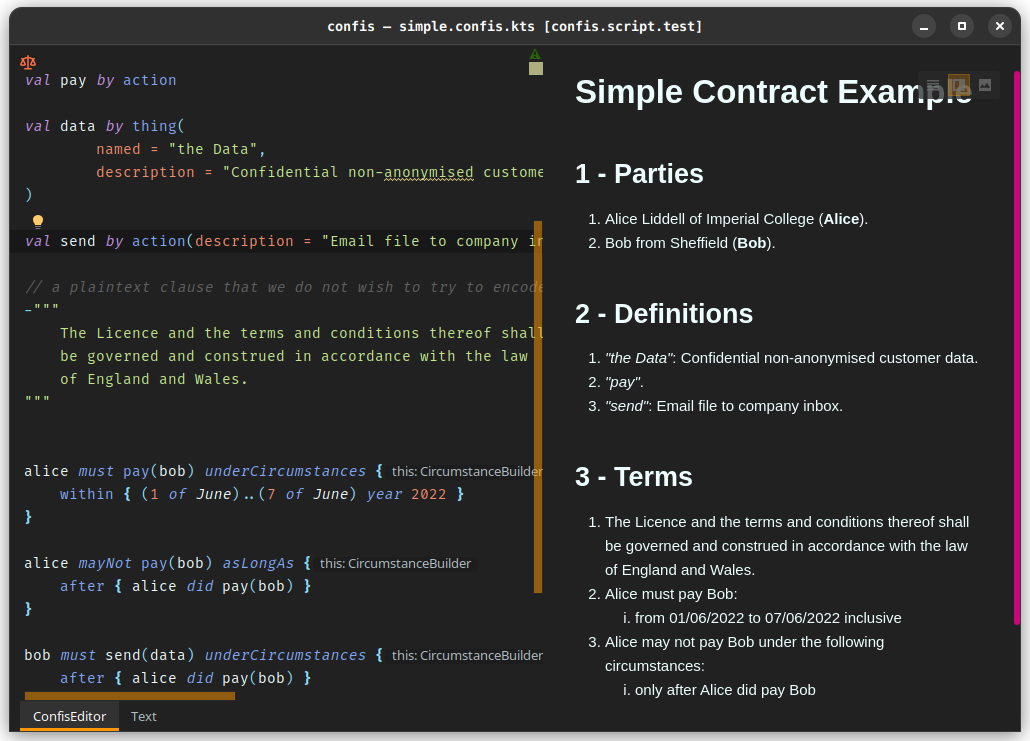
\includegraphics[width=\textwidth]{figures/simple.confis.editor}
    \caption{Screenshot of the Confis Editor, including the legal prose preview}
    \label{fig:confis.minimal.editor}
\end{figure}



For the sake of brevity, this report will omit the implementation details of the live preview -- but a starting point can be found in the software archive under the \texttt{ConfisEditor} class.


\section{Language Documentation}\label{sec:language-documentation}

In the spirit of Software Engineering principles and to further work towards meeting the~\nameref{def:accessibility} requirement, this project also introduces a documentation website, which can be found at \href{https://confis.dcotta.eu}{\texttt{confis.dcotta.eu}} and is pictured in~\autoref{fig:online-docs}.
It is implemented as a series of Markdown documents rendered as HTML pages thanks to the MkDocs~\cite{mkDocs} tool.

\begin{figure}[h]
    \centering
    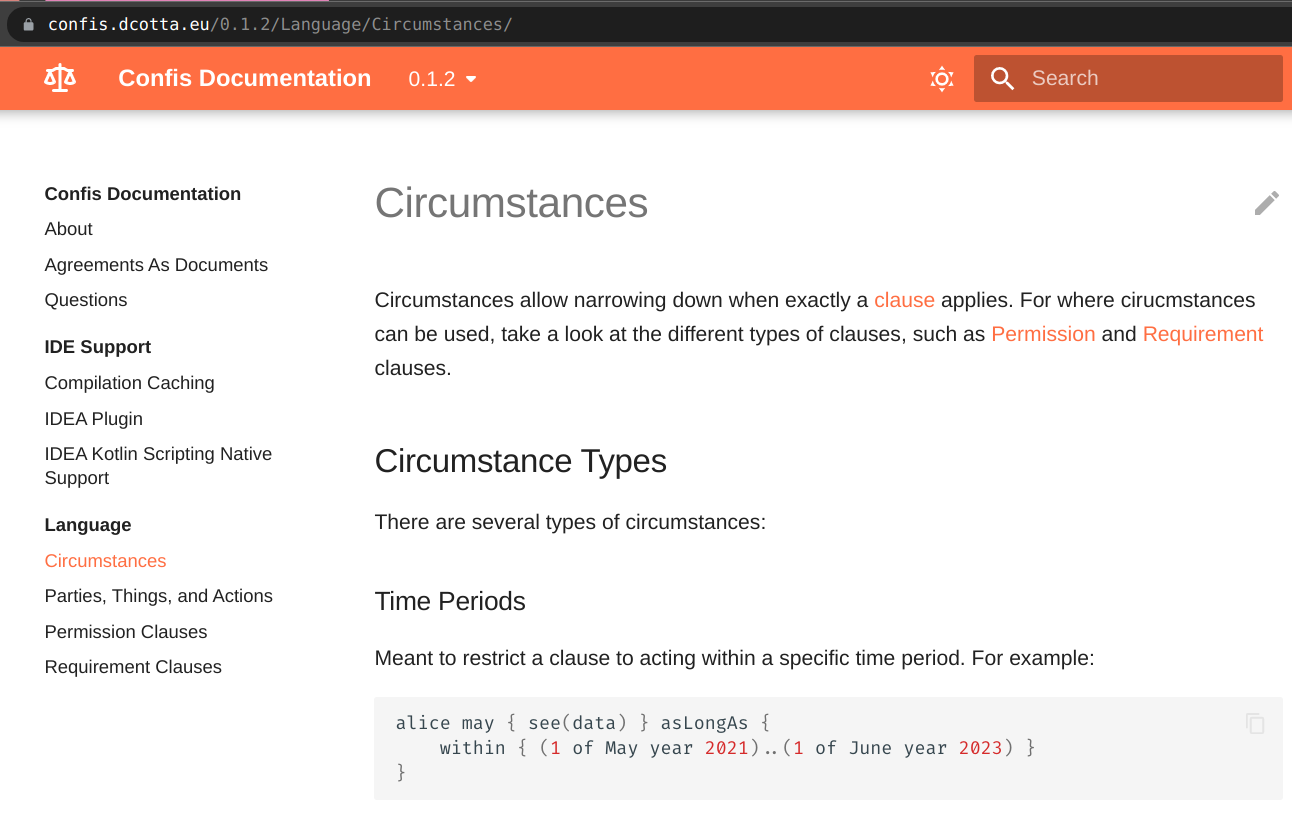
\includegraphics[width=\textwidth]{figures/online-docs}
    \caption{Screenshot of the Circumstances section of the Confis online documentation}
    \label{fig:online-docs}
\end{figure}

The documentation's main aim is to clearly explain~\autoref{sec:language-semantics} without getting into implementation details, nor the specifics of how Circumstances are formalised.


